% Illustrations use the numerical examples in the text.
\newcommand{\FirstIsomorphismFigure}{%
\begin{fig}
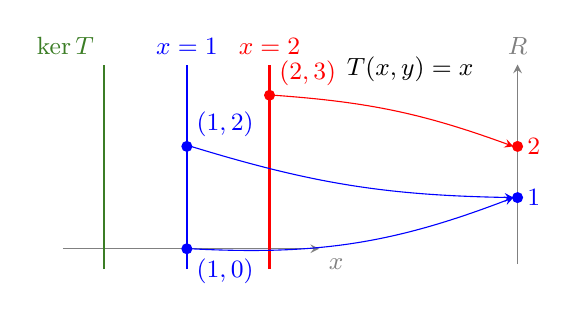
\begin{tikzpicture}[x=1.05cm,y=.65cm,>=stealth,font=\small]
\draw[->,gray](-.5,0)--(2.6,0)node[below right]{$x$};
\draw[OliveGreen,thick](0,-.4)--(0,3.6)node[above left]{$\ker T$};
\draw[blue,thick](1,-.4)--(1,3.6)node[above]{$x=1$};
\draw[red,thick](2,-.4)--(2,3.6)node[above]{$x=2$};
\fill[blue](1,0)circle(2pt)node[below right]{$(1,0)$};
\fill[blue](1,2)circle(2pt)node[above right]{$(1,2)$};
\fill[red](2,3)circle(2pt)node[above right]{$(2,3)$};
\draw[->,gray](5,-.3)--(5,3.6)node[above]{$\mathbb R$};
\fill[blue](5,1)circle(2pt)node[right]{$1$};
\fill[red](5,2)circle(2pt)node[right]{$2$};
\draw[->,blue](1.05,0)to[bend right=12](4.95,1);
\draw[->,blue](1.05,2)to[bend right=8](4.95,1);
\draw[->,red](2.05,3)to[bend left=8](4.95,2);
\node at(3.7,3.5){$T(x,y)=x$};
\end{tikzpicture}
\figcap{The two blue inputs differ by $(0,2)\in\ker T$ and both map to $1$. Each vertical coset has one common output. The induced map sends the blue coset to $1$ and the distinct red coset to $2$.}
\end{fig}}
\newcommand{\NestedQuotientFigure}{%
\begin{fig}
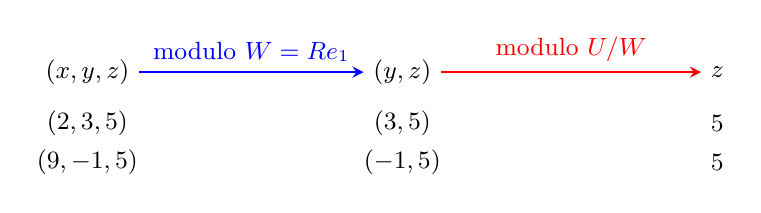
\begin{tikzpicture}[>=stealth,font=\small]
\node (a)at(0,0){$(x,y,z)$};
\node (b)at(4,0){$(y,z)$};
\node (c)at(8,0){$z$};
\draw[->,thick,blue](a)--node[above]{modulo $W=\mathbb Re_1$}(b);
\draw[->,thick,red](b)--node[above]{modulo $U/W$}(c);
\node at(0,-.65){$(2,3,5)$};\node at(4,-.65){$(3,5)$};\node at(8,-.65){$5$};
\node at(0,-1.15){$(9,-1,5)$};\node at(4,-1.15){$(-1,5)$};\node at(8,-1.15){$5$};
\end{tikzpicture}
\figcap{For $W=\mathbb Re_1\subset U=\operatorname{span}(e_1,e_2)$, the first quotient identifies changes in $x$, and the second identifies changes in $y$. Both displayed inputs therefore give the same final coset, determined by $z=5$, just as in $V/U$.}
\end{fig}}
\newcommand{\DualBasisFigure}{%
\begin{fig}
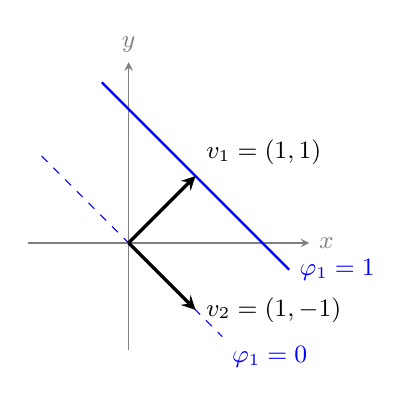
\begin{tikzpicture}[x=.85cm,y=.85cm,>=stealth,font=\small]
\draw[->,gray](-1.5,0)--(2.7,0)node[right]{$x$};
\draw[->,gray](0,-1.6)--(0,2.7)node[above]{$y$};
\draw[blue,dashed](-1.3,1.3)--(1.4,-1.4)node[below right]{$\varphi_1=0$};
\draw[blue,thick](-.4,2.4)--(2.4,-.4)node[right]{$\varphi_1=1$};
\draw[->,very thick](0,0)--(1,1)node[above right]{$v_1=(1,1)$};
\draw[->,very thick](0,0)--(1,-1)node[right]{$v_2=(1,-1)$};
\end{tikzpicture}
\qquad
$\begin{array}{c|cc}
&v_1&v_2\\\hline
\varphi_1=(x+y)/2&1&0\\
\varphi_2=(x-y)/2&0&1
\end{array}$
\figcap{The blue lines are sets where $\varphi_1$ has a fixed value. This functional reads the $v_1$ coefficient: it is $1$ at $v_1$ and $0$ at $v_2$. The table gives both dual functionals and all their defining basis values.}
\end{fig}}
